\documentclass[twoside]{tufte-book}
\hypersetup{colorlinks}

\usepackage[english]{babel}
\usepackage[utf8x]{inputenc}
\usepackage{amsmath}
\usepackage{graphicx}
\usepackage{multicol}
\usepackage[parfill]{parskip}
\usepackage{amssymb}
\usepackage{empheq,amsthm}
\usepackage{xcolor}
\usepackage{cancel}
\usepackage{hyperref}
\usepackage{enumitem}

\setcounter{secnumdepth}{2}
\setcounter{tocdepth}{1}

\newcommand{\degr}{\ensuremath{^\circ}}
\newcommand{\htab}{\hspace{0.5cm}}
\newcommand{\hhtab}{\htab\htab}
\newcommand{\where}{\htab\text{where }}
\newcommand{\andd}{\htab\text{and}\htab}
\newcommand{\so}{\hspace{0.25cm}\ensuremath{\Longrightarrow}\hspace{0.25cm}}

\newcommand{\kcol}[1]{\textcolor{teal}{#1}}
\newcommand{\mcol}[1]{\textcolor{red}{#1}}

\newcommand{\der}[2]{\frac{d#1}{d#2}}
\newcommand{\dder}[2]{\frac{d^2#1}{d#2^2}}


\title[PHYS~232: Waves Study Notes]{%
	\setlength{\parindent}{0pt}%
	PHYS~232: \par Heat \& Waves}
\gdef\subtitle{Waves Study Notes}
\author[Luke~Zhou]{Luke~Zhou}
\gdef\institution{Based on a course given @ McGill University}
\date{Winter 2013 \& Summer 2023}

\renewcommand{\maketitlepage}[0]{%
	{%
		\rmfamily%
		\begin{fullwidth}%
			\fontsize{22}{20}\selectfont\par\noindent\textcolor{darkgray}{{\thanklessauthor}}%
			\vspace{11.5pc}%
			\fontsize{36}{40}\selectfont\par\noindent\textcolor{darkgray}{{\thanklesstitle}}%
			\fontsize{30}{40}\selectfont\par\noindent\textcolor{darkgray}{{\subtitle}}%
			\vfill%
			\fontsize{18}{16}\selectfont\par\noindent\textcolor{darkgray}{{\institution}}%
			\fontsize{18}{16}\selectfont\par\noindent\textcolor{darkgray}{{\thedate}}%
		\end{fullwidth}%
	}
	\thispagestyle{empty}%
	\clearpage%
}

\titleformat{\chapter}%
{\huge\rmfamily\itshape\color{black}}% format applied to label+text
{\llap{\colorbox{black}{\parbox{1.5cm}{\hfill\itshape\huge\color{white}\thechapter}}}}% label
{4pt}% horizontal separation between label and title body
{}% before the title body
[]% after the title body

\titleformat{\section}%
{\LARGE\rmfamily\itshape\color{black}}% format applied to label+text
{\llap{\colorbox{darkgray}{\parbox{1.5cm}{\hfill\itshape\LARGE\color{white}\thesection}}}}% label
{4pt}% horizontal separation between label and title body
{}% before the title body
[]% after the title body

\titleformat{\subsection}%
{\Large\rmfamily\itshape\color{black}}% format applied to label+text
{\llap{\colorbox{lightgray}{\parbox{1.5cm}{\hfill\itshape\Large\color{black}\thesubsection}}}}% label
{4pt}% horizontal separation between label and title body
{}% before the title body
[]% after the title body

\def\mathnote#1{%
	\tag*{\rlap{\hspace\marginparsep\smash{\parbox[t]{\marginparwidth}{%
					\footnotesize[#1]}}}}
}

\let\cleardoublepage=\clearpage
\setlist[itemize]{leftmargin=1cm}


\begin{document}
\maketitlepage

\frontmatter
\tableofcontents 

\mainmatter 

\setlength{\parindent}{0pt}
\raggedbottom

\chapter{Periodic Motion}
\section{Simple Harmonic Motion}
\begin{align*}
\shortintertext{Restoring forces for a displacement $x$:} 
F(x) &= -(k_1 + k_2x^2 + k_3x^3 + \cdots) 
\intertext{For small x, the upper order terms are negligible:} 
F(x) &= -k_1x 
\end{align*}
 
When a small mass is attached to the end of a massless spring:
\[ \boxed{-k_1x = m\frac{d^2x}{dt^2}} \] 

The solution to the differential equation gives a \textbf{sinusoidal} function: \[ \boxed{x = A \sin(\omega t+\varphi_0)} \] %
\begin{center} 
where \textbf{angular frequency} $\boxed{\omega = \sqrt{k_1/m}}$ \textit{(independent of A and $\varphi_0$)}

Period: $T=\frac{2\pi}{\omega} $; Frequency: $f = \frac{1}{T}=\frac{\omega}{2\pi} $   \\
\end{center}


Real vibrations don't go on forever; SHM models a \textbf{steady state of vibration}.

More conditions for using a sinusoidal SHM model:
\begin{itemize}
\item Small amplitudes
\item Simple systems
\item No damping
\item $F_{restoring} \propto x$ %
\end{itemize} 

\section{Rotating Vector Representation}
Represent SHM as the geometrical projection of the \textit{x-component} of uniform circular motion (use polar coordinates, where CCW is positive):
\begin{empheq}[left=\empheqlbrace]{align*}
\theta &= \omega t + \alpha \\
x&=A\cos\theta=A\cos(\omega t + \alpha)
\end{empheq}

Trig identity to convert from cos to sin: \[ \cos\theta=\sin\left(\theta + \frac{\pi}{2}\right) \]
%\[ \leadsto \varphi_0 = \alpha + \frac{\pi}{2} \]
%
\subsection{Extra axis}
\begin{empheq}[right=\empheqrbrace]{align*}
\text{Only \textit{x} is the \textit{measureable} component: } x &= r\cos\theta \\
\text{The y-component is \textit{ficticious}: } y &= r\sin\theta
\end{empheq}

\subsection{Rotations with $j$} 
\begin{align*} %
\mathbf{r}&=\mathbf{i}x+\mathbf{j}y  \\
\text{Rewrite as } \mathbf{r}&=x+\mathbf{j}y 
\end{align*}
Reinterpret $\mathbf{j}y$ as ``move a dist of \textit{y} along the y-axis"

Remove vector notation: \[ \boxed{z=x+jy} \]
Reinterpret $\mathit{j}$ as \textit{``90$^\circ$ rotation CCW from x-axis"} 

So, $\mathit{j^2}$ represents two 90$^\circ$ rotations CCW from x-axis.
\[ \boxed{j^2=-1; j=\sqrt{-1}} \]

Thus, $z=x+jy$ can be considered:
\begin{itemize}
\item Geometrically: as a vector of length $x=\sqrt{x^2+y^2}$ at an angle $\theta = \arctan(\frac{y}{x})$ to the x-axis
\item As a complex \# (with $j$)
\end{itemize}

\section{The Complex Exponential}
General Taylor series: $f(x)=\sum_{n=0}^\infty \frac{x^n}{n!} f^{(n)}(0)$ 

Use Taylor series for sin \& cos to obtain: 
\[ \cos\theta + j\sin\theta = 1+j\theta+\frac{(j\theta)^2}{2!}+\frac{(j\theta)^3}{3!}+\dots+\frac{(j\theta)^n}{n!}+\dots \]

Then, using the Taylor series for $e^{j\theta}$, we obtain a result known as \textbf{Euler's identity}:
\begin{equation}
	\boxed{\cos\theta + j\sin\theta = e^{j\theta}} \label{ch1:eq-eulers-identity}
\end{equation}

To \textit{rotate} the vector rep'd by complex \# $z$ an angle of $+\theta$, multiply by $\boxed{e^{j\theta}}$.

\subsection{Derivatives}
When analyzing periodic displacements, sometimes we get a differential equation of motion with terms involving the velocity \&/or acceleration.

Using the trigonometric functions:
\begin{empheq}[right=\empheqrbrace]{align*}
x&=A \cos(\omega t+\alpha) \\
\frac{dx}{dt}&=-\omega A \sin(\omega t+\alpha) \\
\frac{d^2x}{dt^2}&=-\omega^2 A \cos(\omega t+\alpha) 
\end{empheq}
Leads to an awkward mix of sin \& cos terms when the derivatives are subbed into the differential equation.

Using the complex exponential:
\begin{empheq}[right=\empheqrbrace]{align*}
z=A \cos(\omega t+\alpha)+jA \sin(\omega t+\alpha) &= Ae^{j(\omega t+\alpha)} \\
\frac{dz}{dt}=j\omega Ae^{j(\omega t+\alpha)} &= j\omega z \\
\frac{d^2z}{dt^2}=(j\omega)^2 Ae^{j(\omega t+\alpha)} &= -\omega^2 z 
\end{empheq}

Each $\frac{d}{dt}$ creates a phase shift of $+\pi/2$ (graphically, the vector undergoes a rotation). 

Physically meaningful projections of the complex exponential's derivatives: 
\[ x=\Re(z)  \hhtab \frac{dx}{dt}=\Re(j\omega z) \hhtab \frac{d^2x}{dt^2} = \Re(-\omega^2 z)\]



\section{Small angle approximations}
When $\theta$ is small and measured in radians,
\begin{align}
	\sin\theta &\approx \theta \label{ch1:eq-small-angle-sin} \\
	\tan\theta &\approx \theta  \label{ch1:eq-small-angle-tan} \\
	\cos\theta &\approx 1-\frac{\theta^2}{2} \label{ch1:eq-small-angle-cos}
\end{align}
\chapter{Superposition of Periodic Motions}
The resultant of 2+ harmonic oscillators is the sum of the individual vibrations, if the system is \textbf{linear} (that is, if $F_{restoring}\propto x$).

\section{In 1D}

\subsection{Two Vibrations of Same Frequency}
Consider:
\begin{empheq}[left=\empheqlbrace]{align*}
OP_1: x_1&=A_1\cos(\omega t + \alpha_1) \\
OP_2: x_2&=A_2\cos(\omega t + \alpha_2)
\end{empheq}
Combined vibration: \[ OP: x = A\cos(\omega t+\alpha) \]

All 3 vectors $OP_1, OP_2$ \& $OP$ rotate at the same frequency. 

Let $\beta = \angle P_1OP$.

Phase constant of the combined vib'n: $\alpha = \alpha_1 + \beta$

\paragraph{Using complex exponentials}
\begin{align*}
z = z_1 + z_2 &= A_1 e^{j(\omega t+\alpha_1)} + A_2 e^{j(\omega t+\alpha_2)} \\
&=e^{j(\omega t+\alpha_1)}[A_1 + A_2e^{j(\alpha_2 - \alpha_1)}]
\end{align*}

\paragraph{Special Case: Equal Amplitudes} 
Let \textbf{phase difference} $\delta = \alpha_2-\alpha_1$ \\
From geometry: $ A=2A_1\cos\beta = 2A_1\cos(\delta/2)$

Application: alternating maxima/minimae superposition pattern from two sources converging at a far away point, at any point on line $OB$ (as shown).

\subsection{Two Vibrations of Different Frequencies}
Let the initial phase shifts of both vibrations be zero.
Consider:
\begin{empheq}[left=\empheqlbrace]{align*}
x_1&=A_1\cos(\omega_1 t) \\ 
x_2&=A_2\cos(\omega_2 t)
\end{empheq}

Combined vibration displacement $OX$: \[ 0 \leq OX \leq A_1+A_2 \]

The combined motion will only be periodic if the periods of the component vibrations are \textbf{commensurable} - i.e. $\exists  (n_1$ \& $n_2)\in \mathbb{Z} $ such that $ T = n_1 T_1 = n_2 T_2 $ (use the smallest values of $n_1$ \& $n_2$ possible). 

\paragraph{Beats}  
If the two frequencies are close in frequency: \textbf{beats} will be produced.

Combined vibration will be a disturbance with $\omega=\frac{\omega_1+\omega_2}{2}$, but with an \textit{amplitude that varies periodically with time}.

Add the $x_1$ \& $x_2$ from above. Use the trig identities for $\cos(\theta+\varphi)$ and $\cos(\theta-\varphi)$ to yield:
\[ x = 2A\cos\left(\frac{\omega_1-\omega_2}{2} t\right)\cos\left(\frac{\omega_2+\omega_1}{2} t\right) \]
This is only physically meaningful if $|\omega_1-\omega_2| \ll |\omega_1+\omega_2|$.

Combined displacement can be fitted within an envelope:
\[ x = \pm 2A\cos\left(\frac{\omega_1-\omega_2}{2} t\right) \]

Node-to-node (see diagram): this is half a cycle (a time equal to $\frac{2\pi}{|\omega_1-\omega_2|}$.) \\
So, the aurally observed \textbf{beat frequency} is $|\omega_1-\omega_2|$.

\subsection{Many Vibrations of Same Frequency \& Amplitude}
Let the component vibrations have equal, successive phase differences ($\delta$):
\[ x = A_0\cos(\omega t) \]
Resultant: \[ X = A\cos(\omega t + \alpha) \]

The combining vectors form a polygon that can be inscribed inside a circle.
Each $A_0$ subtends an angle of $\delta$. The resultant vector $A$ subtends an angle $N\delta$.
So:
\begin{empheq}[left=\empheqlbrace]{align*}
A &= N\delta=2R\sin(N\delta/2) \\
A_0 &= 2R\sin(\delta/2) 
\end{empheq}

Solve to get: 
\[ A =A_0 \frac{\sin(N\delta/2)}{\sin(\delta/2)} \] 

\begin{align*}
\intertext{Phase angle $\alpha$ of the combined oscillation: angle between resultant vector \& the 1st vector}
\alpha &= \angle COB - \angle COP \\
&= (90\degr - \delta/2)-(90\degr - N\delta/2) \tag{By properties of isosceles triangles} \\
&= \frac{(N-1)\delta}{2}
\end{align*}

Putting it all together:
\[ \boxed{X = A_0 \frac{\sin(N\delta/2)}{\sin(\delta/2)} \cos\left[\omega t + \frac{(N-1)\delta}{2}\right]} \]

\section{In 2D: Two Vibrations at $\perp$ Angles}
The resultant motion has \textit{two} real components - $x$ and $y$:
\begin{empheq}[left=\empheqlbrace]{align*}
x&=A_1 \cos(\omega t) \\
y&=A_2 \cos(\omega t + \delta)
\end{empheq}

Depending on the value of $\delta$, we'll get different path patterns described by these \textit{parametric equations}. (Be mindful of the direction of tracing - CCW or CW.)

(Study the analytical/mathematical and semicircle-sketching methods to determine the pattern)

\paragraph{Different Frequencies: Lissajous Figures} 
The patterns depend on the $\omega_1:\omega_2$ ratio.
If $\omega_1$ and $\omega_2$ are not \textit{commensuable}, a periodically repeating pattern will not be produced.
\chapter{Free Vibrations}

\section{Overview}
Any physical system that undergoes SHM is associated with...
\begin{itemize}
	\item a constant representing the \kcol{elasticity} of the system $\longrightarrow$ kinetic energy
	\item a constant representing the \mcol{inertia} of the system $\longrightarrow$ potential energy
\end{itemize}

Consider the motion of a mass $m$ on a spring with spring constant $k$:
\begin{align}
	\text{From Newton's Law: }&
	\mcol{m}\ddot{x} + \kcol{k}x = 0 \label{ch3:eq-NL} \\
	\text{From Conservation of Energy: }&
	\frac{1}{2}\mcol{m}\dot{x}^2 + \frac{1}{2}\kcol{k}x^2 = E \label{ch3:eq-CE}
\end{align}

Any equation matching either of the forms above\footnote{\eqref{ch3:eq-CE} also happens to be the \textit{first integral} of  \eqref{ch3:eq-NL}.} automatically has as a solution:
\begin{equation}
\boxed{x = A \cos(\omega t+\alpha)\where\omega^2 = \frac{\kcol{k}}{\mcol{m}}} \label{ch3:eq-SHM-soln}
\end{equation}

Some of the \textbf{simple harmonic oscillators} (SHO) in this chapter are analyzed through comparison with \eqref{ch3:eq-NL}, while others, with \eqref{ch3:eq-CE}.

Although the systems have differing elastic and inertial constants, it will always be true that:
\begin{equation}
	\boxed{
		\omega^2 = \frac{\kcol{\text{elasticity}}}{\mcol{\text{inertia}}} \hhtab 
		T = \frac{2\pi}{\omega} \hhtab 
		f = \frac{\omega}{2\pi}}
\end{equation}

\subsection{Systems analyzed using a force equation}
\begin{center}
	\renewcommand{\arraystretch}{2.5}
\begin{tabular}{lll}
	\hline
	Type of system & Force equation & $\omega^2$ \\ \hline
	Mass on spring &
		$\mcol{m}\ddot{x} + \kcol{k}x = 0$ &
		$\dfrac{\kcol{k}}{\mcol{m}}$
		\\
	\parbox{4cm}{\hyperref[ch3:sec-wire]{Mass on wire} \\\footnotesize{(with Young's Modulus $Y$)}} &
		$\mcol{m}\ddot{x} + \kcol{\frac{AY}{l_0}}x = 0$ &
		$\dfrac{\kcol{AY}}{\kcol{l_0}\mcol{m}} = \dfrac{g}{h}$ 
		\\
	\hyperref[ch3:sec-floating]{Floating objects} &
		$\mcol{m}\ddot{y} + \kcol{g\rho A}y = 0$ &
		$\dfrac{\kcol{g\rho A}}{\mcol{m}} = \dfrac{g}{h}$ 
		\\
	\hyperref[ch3:sec-torsional]{Torsional oscillations} &
		$\mcol{I}\ddot{\theta} + \kcol{c}\theta = 0$ &
		$\dfrac{\kcol{c}}{\mcol{I}}$ 
		\\
	\parbox{3.5cm}{\hyperref[ch3:sec-air]{Spring of air} \\\footnotesize{(isothermal conditions)}} &
		$\mcol{m}\ddot{y} + \kcol{\frac{Ap}{l}}y = 0$ &
		$\dfrac{\kcol{Ap}}{\kcol{l}\mcol{m}}$ 
		\\
	\parbox{3.5cm}{\hyperref[ch3:sec-air]{Spring of air} \\\footnotesize{(adiabatic conditions)}} &
		$\mcol{m}\ddot{y} + \kcol{\frac{A\gamma p}{l}}y = 0$ &
		$\dfrac{\kcol{A\gamma p}}{\kcol{l}\mcol{m}}$ 
		\\
	\hline
\end{tabular}
\renewcommand{\arraystretch}{1}
\end{center}


\subsubsection{Effects of gravity}

\begin{figure}[h]
	\centering
	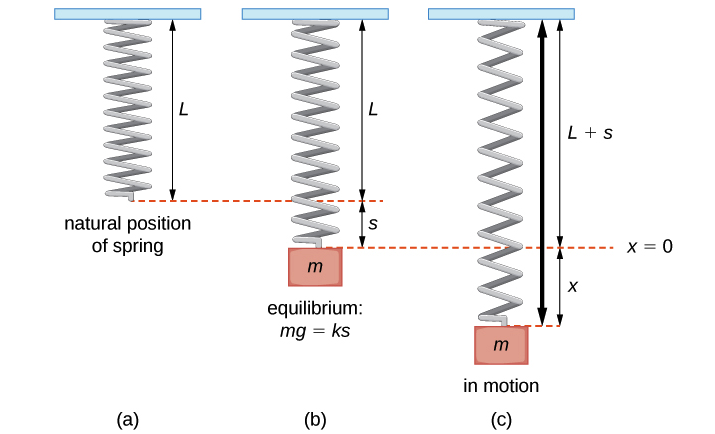
\includegraphics[scale=0.4]{phys232/Ch3-g-new-eqm} \caption{Gravity shifts the equilibrium position of a SHO by a distance $h$.}\label{ch3:fig-g-new-eqm-pos}
\end{figure}

Gravity only changes the equilibrium position of a SHO, without changing the amplitude, period, or frequency:
\begin{align*}
	F_\text{net} &= -F_\text{restoring} + F_g \\
	m\ddot{x} &= -kx + mg \\
	& = -k(x - \frac{mg}{k}) \\
	& = -k(x - h) \where h=\frac{mg}{k}
\end{align*}
Let $y=x-h$. This implies $\ddot{y} = \ddot{x}$. Therefore,
\begin{align*}
	&m\ddot{y} = -ky \\
	&m\ddot{y} + ky = 0  \Longrightarrow \text{still SHM!}
\end{align*}

We can interpret $h$ as the change in position that occurs when the mass is first hung or the floating object is first placed in a liquid and the system reaches \emph{static equilibrium} (see Figure \ref{ch3:fig-g-new-eqm-pos}).
\[ F_g = F_\text{restoring}\Longrightarrow mg = kh \Longrightarrow h = \frac{mg}{k} \]


\subsection{Systems analyzed using the conservation of energy}
\begin{center}
	\renewcommand{\arraystretch}{2.5}
	\begin{tabular}[t]{lll}
		\hline
		Type of system & Energy equation & $\omega^2$ \\ \hline
		Mass on spring &
			$\frac{1}{2}\mcol{m}\dot{x}^2 + \frac{1}{2}\kcol{k}x^2 = E $ &
			$\dfrac{\kcol{k}}{\mcol{m}}$
			\\
		\hyperref[ch3:sec-simple-pendulum]{Simple pendulum} &
			$\frac{1}{2}\mcol{I}\dot{\theta}^2 + \frac{1}{2}\kcol{mgl}\theta^2 = E $ &
			$\dfrac{\kcol{mgl}}{\mcol{I}} = \dfrac{\kcol{mgl}}{\mcol{ml^2}}= \dfrac{\kcol{g}}{\mcol{l}}$ 
			\\
		\parbox{5.5cm}{	\hyperref[ch3:sec-complex-pendulum]{Arbitrary pendulum} \footnotesize(with radius of gyration $k$, centre of mass at distance $h$ from point of suspension)}&
			$\frac{1}{2}\mcol{m(k^2+h^2)}\dot{\theta}^2 + \frac{1}{2}\kcol{mgh}\theta^2 = E $ &
			$\dfrac{\kcol{gh}}{\mcol{k^2+h^2}}$ 
			\\
		\hyperref[ch3:sec-uTube]{Water in a U-tube} &
			$\frac{1}{2}\mcol{\rho Al}\dot{y} + \frac{1}{2}\kcol{(2g\rho A)}y^2 = E$ &
			$\dfrac{\kcol{2g}}{\mcol{l}}$ 
			\\
		\hyperref[ch3:sec-torsional]{Torsional oscillations} &
			$\frac{1}{2}\mcol{I}\dot{\theta} + \frac{1}{2}\kcol{c}\theta^2 = E$ &
			$\dfrac{\kcol{c}}{\mcol{I}}$ 
			\\
		\parbox{5cm}{	\hyperref[ch3:sec-massive-springs]{Massive springs} \\\footnotesize{(with mass $M$)}} &
			$\frac{1}{2}\mcol{\left(m + \frac{1}{3}M \right)}\dot{x} + \frac{1}{2}\kcol{k}x^2 = E$ &
			$\dfrac{\kcol{k}}{\mcol{m + M/3}}$ 
			\\
		\hline
	\end{tabular}
	\renewcommand{\arraystretch}{1}
\end{center}


\section{Solving for the equation of motion of a harmonic oscillator}

\begin{proof}[Solving for the solution]
Rewrite \eqref{ch3:eq-NL} in terms of $k/m$:
\begin{align}
m\ddot{x} + kx &= 0 \notag\\
\ddot{x} + \frac{k}{m}x &= 0 \notag\\
\ddot{x} + \omega^2 x  &= 0 \label{ch3:eq-xdd}
\end{align}

\eqref{ch3:eq-xdd} implies $\ddot{x}$ is a multiple of $x$. This is a property of the exponential function, so write: 
\begin{equation}
	x=Ce^{pt} \label{ch3:eq-xCPT}
\end{equation}
where $p$ is a dimensional constant such that $pt$ is dimensionless, and $C$ is a coefficient.
%
\begin{align*}
\intertext{Sub \eqref{ch3:eq-xCPT} back into \eqref{ch3:eq-xdd}:}
\frac{d^2}{dt^2}(Ce^{pt})+\omega^2(Ce^{pt}) &= 0\\
p^2Ce^{pt}+\omega^2Ce^{pt}&=0 \\
Ce^{pt}(p^2+\omega^2) &=0 \\
\Longrightarrow p^2 + \omega^2 &= 0 \\
p^2 &= -\omega^2 \\
p &= \pm j\omega
\end{align*}

Because we have two possibilities for $p$, our solution to \eqref{ch3:eq-xdd} could have been written more generally as:
\[ x = C_1e^{j\omega t}+C_2e^{-j\omega t} \]


Geometrically, $x$ is the sum of two vectors: one with length $C_1$ rotating CCW and another with length $C_2$ going CW, both with the same angular displacement $\omega t$ (see Figure~\ref{ch3:fig-complex-sols}a).

In order to produce a harmonic oscillation along the $x$-axis, the $y$-components of the vectors must cancel. This is also the case when we have an initial phase angle $\alpha\neq 0$ (see Figure~\ref{ch3:fig-complex-sols}b).

\begin{figure}[h]
	\centering
	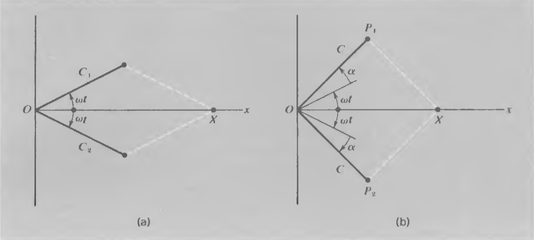
\includegraphics[scale=0.7]{phys232/Ch3-adding-complex-solutions.png} \caption{Superposition of complex solutions of \eqref{ch3:eq-xdd} with (a) $\alpha=0$ and (b) $\alpha\neq 0$. For $OX$ to be a harmonic oscillation, $C1=C2$.}\label{ch3:fig-complex-sols}
\end{figure}


For the $y$-components to cancel, we need $C_1=C_2$. Hence\footnote{Reminder: $\cos(-\theta)=cos\theta$ and $\sin(-\theta)=-\sin\theta$},
\begin{align*}
x
&=Ce^{j(\omega t +\alpha)} + Ce^{-j(\omega t +\alpha)} \\
&=C[\cos(\omega t + \alpha) + j\sin(\omega t + \alpha) + \cos(-(\omega t + \alpha)) + j\sin(-(\omega t + \alpha))] \\
&=C[\cos(\omega t + \alpha) + \cancel{j\sin(\omega t + \alpha)} + \cos(\omega t + \alpha) - \cancel{j\sin(\omega t + \alpha)}] \\
&= 2C\cos(\omega t + \alpha) \\
\therefore
x &= Acos(\omega t + \alpha) \where A=2C
\end{align*}

This is why, for SHM in general, we can assume solutions of the type:
\begin{equation}
	x=\Re(z) \where z=Acos(\omega t + \alpha)
\end{equation}
\end{proof}


\section{Elastic Wire \& Young's Modulus} \label{ch3:sec-wire}

Apply a force $F_\text{app}$ to one end (e.g., by hanging a mass off it) and let the other end remain fixed. When the wire/rod is in \textit{static equilibrium}, let us define two quantities:

\[ \text{stress} = \frac{F_\text{app}}{A} \where\text{$A$ is the cross-sectional area} \]

\[  \text{strain} = \frac{x}{l_0} \where\text{$x$ is the extension of the wire}  \]

The ratio between these two quantities is a constant $Y$, which we call \textbf{Young's modulus of elasticity} for the material\footnote{... as long as the strain is small enough, such that the material is not permanently deformed when stretched.}:
\begin{equation}
	\boxed{ Y = \frac{\text{stress}}{\text{strain}} = \text{const}} \label{ch3:eq-Youngs-Modulus}
\end{equation}

Let us consider the force $F = -F_\text{app}$ exerted \emph{by} the rod \emph{on} another object. Hence,
\begin{align}
	& Y = \frac{-F/A}{x/l_0} \notag \\
	& \boxed{F = \kcol{\frac{-AY}{l_0}} x } \label{ch3:eq-Youngs-F}
\end{align}


Once a mass $m$ is hung on one end:
\[ \omega^2 = \sqrt{\frac{\kcol AY}{\mcol m \kcol{l_0}}} \]

We can rewrite this in terms of properties more easily measured at static equilibrium, such as $h$, the increase of length reached at static equilibrium after the mass is attached.
\[ \mcol{m}g=\kcol{\frac{AY}{l_0}} h \Longrightarrow \frac{ml_0}{AY}=\frac{h}{g} \]
\begin{equation}
\therefore \omega^2 = \frac{g}{h}  \label{ch3:eq-elastic-wire-result}
\end{equation} 

Remark: this result is similar to that for a simple pendulum (Equation~\ref{ch3:eq-simple-pendulum-result}).

\section{Floating Objects} \label{ch3:sec-floating}

\begin{figure}[h]
	\centering
	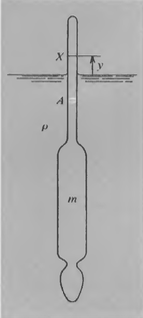
\includegraphics[scale=0.6]{phys232/Ch3-floating.png} \caption{Floating object at a vertical displacement of $y$ from its equilibrium position.}\label{ch3:fig-floating}
\end{figure}

Let the floating object (of mass $m$) have a constant cross-sectional area $A$ parallel to the liquid surface.

Recall:
\[ F_\text{buoyancy} = \text{weight of liquid displaced by the floating object} \]
\[ \boxed{F_b  = \kcol{g\rho A}y} \]

where...
\begin{itemize}
	\item $\rho$: density of the liquid
	\item $y$: vertical displacement of the object above equilibrium position
\end{itemize}


By Newton's Law:
\[ \mcol{m}\frac{d^2y}{dt^2} = -\kcol{g\rho A}y \]
\[ \therefore \omega^2 = \frac{\kcol{g\rho A}}{\mcol{m}} \]

We can, again, rewrite $\omega^2$ in terms of $h$, the change in equilibrium position when the object is placed in the liquid and reaches static eqm:
\[ \mcol{m}\cancel{g}=\kcol{\cancel{g}\rho A} h
\Longrightarrow
h = \frac{m}{\rho A} \]
\[ \therefore \omega^2 = \frac{g}{h} \]


This is analogous to the $\omega^2$ of an elastic wire, seen earlier in \eqref{ch3:eq-elastic-wire-result}. 


\section{The Pendulum}
\begin{figure}[h]
	\centering
	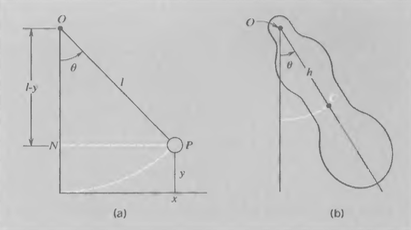
\includegraphics[scale=0.6]{phys232/Ch3-pendulum.png} \caption{(a) Simple pendulum; (b) pendulum of arbitrary shape with its centre of mass at $C$.}\label{ch3:fig-pendulum}
\end{figure}

Let $\theta$ represent the angular displacement of the pendulum. Assume small $\theta$ such that $y \ll x$. 


\subsection{Simple Pendulum} \label{ch3:sec-simple-pendulum}
By the Pythagorean Theorem (see Figure~\ref{ch3:fig-pendulum}):
\begin{align}
l^2 &= x^2 + (l-y)^2  \notag \\	
\cancel{l^2} &= x^2 + \cancel{l^2} - 2ly + y^2 \notag \\
x^2 &= 2ly - {y^2} \notag \\
x^2 &\approx 2ly  \notag \\
\Longrightarrow y &\approx \frac{x^2}{2l} \label{ch3:eq-pendulum-pythag}
\end{align}

In addition,
\begin{equation}
v^2=\left( \frac{dx}{dt} \right)^2 + \left(\frac{dy}{dt} \right)^2
\approx  \left( \frac{dx}{dt} \right)^2 \label{ch3:eq-pendulum-v2}
\end{equation}

By the Conservation of Energy and using the approximations \eqref{ch3:eq-pendulum-pythag} and  \eqref{ch3:eq-pendulum-v2}:
\begin{align}
\frac{1}{2} mv^2 + mgy &= E \notag \\
\frac{1}{2} \mcol{m} \left( \frac{dx}{dt} \right)^2 + \frac{1}{2} \kcol{\frac{mg}{l}} x^2 &= E  \label{ch3:eq-pendulum-E}
\end{align}


We can rewrite this result in terms of $\theta$. Substitute\footnote{Use the small angle approximation $\cos\theta \approx 1-\frac{\theta^2}{2}$, from Equation~\eqref{ch1:eq-small-angle-cos}}:
\begin{equation*}
v = l\left(\frac{d\theta}{dt}\right) \andd
y = l(1-\cos\theta) \approx \frac{1}{2}l\theta ^2
\end{equation*}

So, \eqref{ch3:eq-pendulum-E} becomes:
\begin{equation}
	\frac{1}{2} \mcol{ml^2} \left( \frac{d\theta}{dt} \right)^2 + \frac{1}{2} \kcol{mgl} \theta^2 = E \label{ch3:eq-pendulum-E-theta}
\end{equation}

Both \eqref{ch3:eq-pendulum-E} and \eqref{ch3:eq-pendulum-E-theta} imply that:
\begin{equation}
	\therefore \omega^2 = \frac{g}{l} \label{ch3:eq-simple-pendulum-result}
\end{equation}


\subsection{Pendulum of an Arbitrary Shape} \label{ch3:sec-complex-pendulum}
Let its center of mass $C$ be at a dist $h$ from the point of suspension $O$\footnote{This allows us to find the PE of the pendulum using the height of the CM.}, as shown in Figure~\ref{ch3:fig-pendulum}b.

\subsubsection{With respect to an axis passing through the point of suspension}

Let $I$ represent the moment of inertia \emph{about an axis passing through $O$}. Then:
\begin{equation*}
PE = \frac{1}{2} mgh\theta^2 \andd
KE = \frac{1}{2} I\left( \frac{d\theta}{dt} \right)^2
\end{equation*}
\begin{equation} 
	\Longrightarrow
	\frac{1}{2} \mcol{I}\left( \frac{d\theta}{dt} \right)^2 + \frac{1}{2} \kcol{mgh}\theta^2 = E \label{ch3:eq-pendulumEO}
\end{equation}

\subsubsection{With respect to an axis passing through the centre of mass}
From the \emph{parallel axis theorem} -- for an axis passsing through point $C$, we have:
\begin{align*}
	I_C &= I_\text{CM} + mh^2 \\
	&= mk^2 + mh^2
\end{align*}

where $k$ is the \emph{radius of gyration}\footnote{The radius of gyration $k$ is the length of a simple pendulum that could ``replace" the complex pendulum, while keeping the same mass.}. Thus,
\begin{align*}
	KE_C %&= \frac{1}{2} ( I_\text{CM} + mh^2 ) \left( \frac{d\theta}{dt} \right)^2 \\
	&= \frac{1}{2} m(k^2 + h^2 ) \left( \frac{d\theta}{dt} \right)^2
\end{align*}

Then, \eqref{ch3:eq-pendulumEO} becomes:
\[ \frac{1}{2} \mcol{m(k^2+h^2)} \left( \frac{d\theta}{dt} \right)^2  + \frac{1}{2} \kcol{mgh}\theta^2 = E \]

\begin{equation*}
	\therefore \omega^2 = \frac{\kcol{gh}}{\mcol{m(k^2+h^2)}}
\end{equation*}

This result is analogous to what we found for an elastic wire (Equation~\ref{ch3:eq-elastic-wire-result}).

\section{Liquid in a U-Tube} \label{ch3:sec-uTube}

\begin{figure}[h]
	\centering
	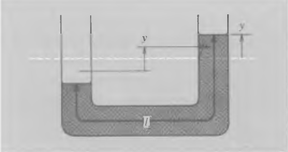
\includegraphics[scale=0.8]{phys232/Ch3-utube.png} \caption{Oscillating liquid column in a U-tube.}\label{ch3:fig-utube}
\end{figure}

Examine the vertical displacement $y$ of the liquid surface from equilibrium in a U-tube with uniform cross-sectional area $A$. Define:
\begin{itemize}
	\item $l$: total length of liquid column
	\item $\rho$: liquid density
\end{itemize}

When liquid \textit{rises} a height of $y$ in one end, the liquid in the other end \textit{sinks} by the same height $y$. The mass of the liquid that moves is $\rho Ay$. 

Assume the whole liquid, which has mass $\rho Al$, moves with speed $dy/dt$. So,
\[ KE = \frac{1}{2} \rho Al \left(\frac{dy}{dx}\right)^2 \andd
PE = g\rho Ay^2 \]
\[ \Longrightarrow \frac{1}{2} \mcol{\rho Al} \left( \frac{dy}{dt} \right)^2 
+ \frac{1}{2} \kcol{(2g\rho A)} y^2 = E  \] 

\begin{equation}
\therefore \omega^2 = \frac{\kcol{2g}}{\mcol{l}} \label{ch3:eq-utube-result}
\end{equation}

Again, the result for a U-tube \eqref{ch3:eq-utube-result} is comparable to that for an elastic wire \eqref{ch3:eq-elastic-wire-result}.

\section{Torsional Oscillations} \label{ch3:sec-torsional}

\begin{figure}
	\centering
	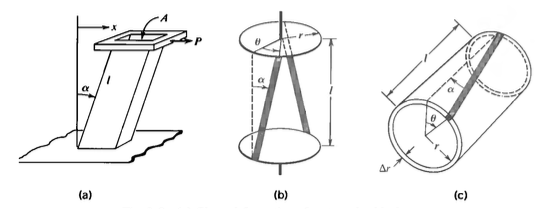
\includegraphics[scale=0.7]{phys232/Ch3-shear-torsion.png} \caption{(a) Shear deformation of a rectantular block; (b) Torque on rectangular strips during shear deformation; (c) A twisted tube can be considered as a collection of strips undergoing shear.}\label{ch3:fig-shear-torsion}
\end{figure}

If the torque $\tau \propto$ angular displacement $\theta$ between two ends of an object,
\[ \tau=-\kcol{c}\theta \where\text{$c$ is the torsion constant of the system.} \]

Stored potential energy: \[ U= -\int \tau d\theta = \frac{1}{2} \kcol{c}\theta^2 \]

If one end has a moment of inertia $\mcol{I}$ and the inertia of the twisted system itself is negligible, then by the conservation of energy:
\[ \frac{1}{2} \mcol{I} \left( \frac{d\theta}{dt}\right)^2 + \frac{1}{2} \kcol{c}\theta^2 = E \]

Thus:
\begin{equation*}
\omega^2 = \frac{\kcol{c}}{\mcol{I}}
\end{equation*}

\subsection{Shear \& the shear modulus}
Apply a horizontal force $F_\text{app}$ to the board in Figure~\ref{ch3:fig-shear-torsion}a. Two of the sides change from rectangles to parallelograms. Define an \textbf{angle of shear, $\alpha$}:
\[ \alpha = \frac{x}{l} \]

It turns out that, just like when we stretch an elastic wire (Section~\ref{ch3:sec-wire}), the ratio between stress and the ``angular strain" is a constant.

We call this the \textbf{shear modulus} or \textbf{modulus of rigidity}, $n$, for the material (cf. Equation~\ref{ch3:eq-Youngs-Modulus}):
\[  n= \frac{F_\text{app}/A}{\alpha} = \text{const} \]

Let us consider the force $F=-F_\text{app}$ exerted \emph{by} the sheared material \emph{onto} the board. Hence,
\[  n = \frac{-F/A}{x/l} \]
\begin{equation}
	\boxed{F = \kcol{\frac{-nA}{l}} x}  \label{ch3:eq-torsional-F}
\end{equation}

Notice that \eqref{ch3:eq-torsional-F} for {shear deformations} is comparable to \eqref{ch3:eq-Youngs-F} for {longitudinal deformations}\footnote{Another modulus also exists: the \textbf{bulk modulus}, $K$, which describes the resistance of a material to changes in volume -- more about this in Section~\ref{ch3:sec-bulk-modulus}.}.

\subsection{Torque due to shear}
Refer to Figure~\ref{ch3:fig-shear-torsion}b, where two disks of radius $r$ on spindles are connected by two rectangular strips of material, each with cross-sectional area $A$.

Twist one spindle through a small $\theta$; the end of each strip undergoes shear through a distance $x=r\theta$. 

Substituting this into \eqref{ch3:eq-torsional-F}, we see that the restoring force $\Delta F$ exerted by each strip tangentially to the disk is:
\[ \Delta F = -\kcol{nA\frac{r}{l}} \theta \]

Hence, there is a restoring torque exerted by \emph{each} strip about the axis of twist:
\begin{align*}
	\Delta\tau &= r\,dF  \notag \\
	&= -\frac{nAr^2\theta}{l} 
\end{align*}

\subsubsection{Thin Walled Tube}
Refer to Figure~\ref{ch3:fig-shear-torsion}c, where we will consider a twisted, thin-walled tube as a collection of many strips, each undergoing shear and contributing restoring torques about the axis of twist.

Let the radius be $r$ and the wall thickness be $\Delta r$. This means the cross-sectional area is $A=2\pi r \Delta r$. The restoring torque from a \emph{thin ring of strips} is thus:
\begin{equation}
\Delta \tau = -\frac{2\pi nr^3\Delta r}{l} \theta  \label{ch3:eq-thinTube_dtau}
\end{equation}

\subsubsection{Solid Tube}
We can model a \textit{solid} tube or cylinder as multiple thin-walled tubes. Integrate \eqref{ch3:eq-thinTube_dtau} to obtain, as a total restoring torque:
\begin{equation*}
	\boxed{\tau = -\kcol{\frac{\pi nr^4}{2l}} \theta}
\end{equation*}

\section{``The Spring of Air"} \label{ch3:sec-air}

\begin{figure}
	\centering
	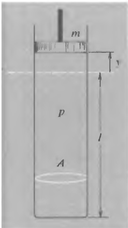
\includegraphics[scale=0.7]{phys232/Ch3-air.png} \caption{Piston in a vertical air column.}\label{ch3:fig-air}
\end{figure}

Consider a closed piston-gas system, as pictured in Figure~\ref{ch3:fig-air} Let $m$ represent the mass of the movable piston, and $p$, the pressure of the gas inside the tube.

When the piston moves a distance of $y$ from equilibrium position $l$, the pressure of the gas changes by $\Delta p$.

\subsection{Isothermal conditions}
Under {isothermal} (constant temperature) conditions, \emph{Boyle's Law} applies:
\begin{align*}
pV &= \text{const} \\
p\Delta V + V\Delta p &= 0 \tag*{(cf. the product rule for differentiation)}
\end{align*}

But... the equilibrium volume was $V = Al$ and the change in volume is $\Delta V = Ay$.
\[ p(Ay) + (Al)\Delta p = 0 \]
\[ \Delta p = -\frac{py}{l} \]

Because $F=PA$:
\begin{equation}
	\boxed{F=-\kcol{\frac{Ap}{l}} y } \label{ch3:eq-pistonF}
\end{equation}

\subsection{Bulk Modulus} \label{ch3:sec-bulk-modulus}

Compare \eqref{ch3:eq-pistonF} with \eqref{ch3:eq-Youngs-F} for stretching a rod. Here, $p$ plays a role analogous to $Y$. We can call $p$ the \textbf{isothermal bulk modulus} of the gas:
\begin{equation*}
	K_\text{isothermal} = p
\end{equation*}

More formally, the \textbf{bulk modulus} of a specimen is defined by:
\begin{align*}
	K &= -\frac{dp}{dV/V} \notag \\
	\Aboxed{K &= -V\frac{dp}{dV}}
\end{align*}

\subsection{Adiabatic conditions}

In general, $K_\text{isothermal}$ is not a good descriptor of the elasticity of an air column.
\begin{itemize}
	\item When a gas is compressed, it becomes \emph{warmer} because of the work being done on it.
	\item Heating results in a greater restoring force.
	\item We expect a higher value than $p$ for the elasticity of the gas.
\end{itemize}

In \textbf{adiabatic conditions} (closed system; no flow of heat in/out of the gas), we have:
\begin{align*}
pV^\gamma &= \text{constant} \\
\Longrightarrow \ln p + \gamma\ln V &= \text{const} \tag{taking $\ln$ of both sides} \\
\Longrightarrow \frac{1}{p}\frac{dp}{dV} + \frac{\gamma}{V} &= 0 \tag{integrating both sides} 
\intertext{By the definition of $K_\text{adiabatic}$,}
K_\text{adiabatic} &= -V \frac{dp}{dV} \\
\Aboxed{K_\text{adiabatic} &= \gamma p}
\end{align*}

Because elasticity is enhanced under adiabatic conditions, and the frequency of vibrations is increased too:
\begin{equation*}
	\therefore
	\omega^2_\text{isothermal} \propto \kcol{p} \andd
	\omega^2_\text{adiabatic} \propto \kcol{\gamma p}
\end{equation*}

\section{Massive Springs} \label{ch3:sec-massive-springs}

\begin{figure}[h]
	\centering
	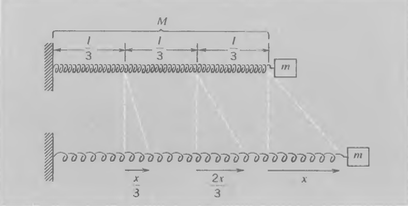
\includegraphics[scale=0.8]{phys232/Ch3-massive-spring.png} \caption{Uniform extension of a massive spring with mass $M$.}\label{ch3:fig-massive-spring}
\end{figure}

Suppose this time the spring itself has a mass of $M$. Suppose that it has a spring contant $k$ and that there is a mass $m$ attached to it. Let the equilibrium length of the spring be $l$.

The \emph{linear mass density} of the spring is $ \lambda = {M}/{l} $.

Consider an infinitesimal segment of the spring initially at a distance $s$ from the fixed end $(0 \leq s \leq l)$, with a width $ds$. Its mass is:
\[ dM = \lambda\,ds = \frac{M}{l}\,ds \] 

\paragraph{Assumption} Each point on the spring undergoes a displacement proportional to its distance from the fixed end (Figure~\ref{ch3:fig-massive-spring}). So, the displacement and speed of the segment are:
\[ \text{displacement} = \frac{s}{l} \, x \andd
\text{speed} = \frac{s}{l} \frac{dx}{dt} 
\]

Its kinetic energy is \[ dK = \frac{1}{2}\left( \frac{M}{l} ds \right) \left( \frac{s}{l} \frac{dx}{dt} \right)^2 = \frac{M}{2l^3} \left( \frac{dx}{dt} \right)^2 s^2 \, ds \]

For the kinetic energy of the whole spring, integrate, treating $dx/dt$ as a constant:
\begin{align*}
K_\text{spring} &= \frac{M}{2l^3} \left( \frac{dx}{dt} \right)^2  \int_0^{l} s^2 \, ds \\
&= \frac{1}{6}M\left(\frac{dx}{dt}\right)^2
\end{align*}

So, the energy-conservation statement for the whole system becomes:
\begin{align*}
\frac{1}{2}m\left(\frac{dx}{dt}\right)^2 + \frac{1}{6}M\left( \frac{dx}{dt}\right)^2 + \frac{1}{2}kx^2 &= E  \\
\frac{1}{2} \mcol{\left( m + \frac{M}{3} \right)} \left(\frac{dx}{dt}\right)^2 + \frac{1}{2} \kcol{k} x^2 &= E
\end{align*}
\[ \therefore \omega^2 = \frac{\kcol{k}}{\mcol{m+M/3}} \]

This is the equivalent of taking a massless spring (see Equation~\ref{ch3:eq-SHM-soln}), and then adding a mass of $m + M/3$ to the end.

In reality, our model holds only when $M \ll m$. Otherwise, the force along the spring is not constant -- we can no longer assume that the elongation of a point is proportional to its distance from the fixed end.

\section{The Decay of Free Oscillations}

In general, resistive forces act in a direction opposite to $\vec{v}$ and have magnitude:
\[ F_b = b_1v + b_2v^2\]

When $v$ is small in comparison to $b_1/b_2$, we can make an approximation:
\begin{equation*}
	\boxed{\vec{F}_b = b\vec{v}}
\end{equation*}

For our mass-spring system with damping, our statement of Newton's Law becomes:
\begin{align*}
	m\ddot{x} &= -kx - bv \\
	m\ddot{x} + b\dot{v} + kx &= 0 \\
	\ddot{x} + \gamma \dot{v} + \omega_0^2 x &= 0
\end{align*}
where
\[ \boxed{\gamma = \frac{b}{m} \andd \omega_0 = \frac{k}{m}} \]

Interpretation:
\begin{itemize}
	\item $\gamma$: damping constant (with dimensions of frequency)
	\item $\omega_0^2$: angular frequency of the system if damping were absent
\end{itemize}

Solution:
\[
\boxed{ x = A e^{-\gamma t/2} \cos(\omega t + \alpha) \where \omega ^2 = \omega_0^2 - \frac{\gamma^2}{4} }
\]

Amplitude:
\[ A(t) = A_0 e^{-\gamma t/2} \]

Total energy:
\[ E(t) = \frac{1}{2}kA^2 = \frac{1}{2}kA_0^2 e^{-\gamma t} = E_0 e^{-\gamma t} \]

Quality value:
\[ Q = \frac{\omega_0}{\gamma} \]

\subsection{Large Damping}
\subsubsection{Overdamping ($ \omega_0 \ll \gamma/2 $)}
\[ x = A_1 e^{-(\gamma/2 + \beta)t} + A_2 e^{-(\gamma/2-\beta)t} \]
where \[ \beta = \left(\frac{\gamma^2}{4}-\omega_0^2 \right)^{1/2} \]

\subsubsection{Critical Damping ($ \omega_0 = \gamma/2 $)}
\[ x = (A + Bt) e^{\gamma t/2}\]
\chapter{Forced Vibrations \& Resonance}

\fbox{
	\begin{minipage}{\linewidth}{
	\linespread{1.5}\selectfont
	
	In this chapter, we consider the effects of a \textbf{driving force} $F(t)$ on a system:
	\[ {F(t) = F_0 \cos(\omega t)} \]
	where...
	\begin{itemize}
		\item $\omega$ represents the \textbf{driving frequency}
		\item $\omega_0$ represents the \textbf{natural frequency} of the system, associated with a \textbf{free vibration} (see Chapter~\ref{ch:free-vibrations})
	\end{itemize}
	}
\end{minipage}}
\vspace{0.5em}

We will see that...
\begin{itemize}
	\item As $\omega \to \omega_0$, the amplitude of oscillation increases
	\item ... whereas as $\omega$ gets farther away from $\omega_0$, the amplitude becomes smaller
	\item This phenomenon is known as \textbf{resonance}.
\end{itemize}

The system will initially have the tendency to vibrate at $\omega_0$, but it will ultimately begin to vibrate at $\omega$. We thus have two stages:
\begin{enumerate}
	\item \textbf{Transient state}: we have a superposition of oscillations at frequencies $\omega$ and $\omega_0$. The free vibration gradually gets damped away until...
	\item \textbf{Steady state}: only the the driving vibration remains, so the system oscillates at $\omega$
\end{enumerate}

\section{Forced Oscillations without Damping: Steady State}
We will consider the \emph{steady state} of a forced oscillation with negligible damping, ignoring the fact that we need damping to get past the transient state.

Force equation:
\begin{align}
	m\ddot{x} &= -kx + F_0 \cos(\omega t)  \notag \\
	\Longrightarrow
	\mcol{m}\ddot{x} + \kcol{k}x &= F_0 \cos(\omega t)	\label{ch4:eq-no-b}
\end{align}

\paragraph{Case (a): $\omega < \omega_0$}
If the driving force's frequency is much lower than the natural frequency...
\begin{itemize}
	\item We expect a low acceleration (since $\ddot{x} \propto \omega^2$).
	\item So, the $\kcol{k}x$ term dominates over $\mcol{m}\ddot{x}$.
	\item The response is controlled by the \kcol{stiffness} of the string.
	\item Since $F_0 \approx kA$, the amplitiude will be $A\approx F_0/k$
\end{itemize}

\paragraph{Case (b): $\omega > \omega_0$}
If the driving force's frequency is much higher than the natural frequency...
\begin{itemize}
	\item We expect a higher acceleration (since $\ddot{x} \propto \omega^2$).
	\item So, the $\mcol{m}\ddot{x}$ term dominates over $\kcol{k}x$.
	\item The response is controlled by the \mcol{inertia} of the string.
	\item We expect a relatively small $A$, opposite in phase with the driving force (since $x$ is 180°  out of phase from $\ddot{x}$)\footnote{Notice that in Figure~\ref{ch4:no-damping-pendula}b, when $F$ is to the left, $x$ is to the right; when $F$ is to the right, $x$ is to the left.}
\end{itemize}

These cases are summarized in Figure~\ref{ch4:no-damping-pendula}.

\begin{figure}[h]
	\centering
	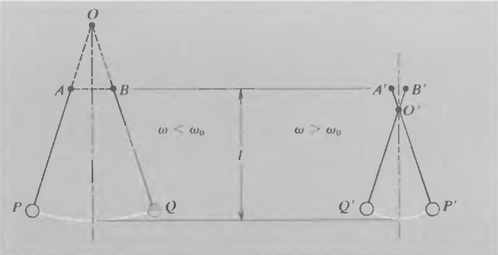
\includegraphics[scale=0.7]{phys232/Ch4-forced-no-damping-pendula.png} 
	\caption{The motion of simple pendula undergoing horizontal forced oscillations when (a) $\omega<\omega_0$ and (b) $\omega>\omega_0$.}\label{ch4:no-damping-pendula}
\end{figure}

\begin{center}
\begin{tabular}{cccc}
	\hline
	\multicolumn{2}{c}{Case} & $A$ & \parbox{3cm}{\centering Phase difference $\alpha$ b/w $x$ \& $F$}  \\
	\hline\hline
	(a) & $\omega < \omega_0$ & large & 0° \\
	(b) & $\omega > \omega_0$ & small & 180° \\
	\hline
\end{tabular}
\end{center}


\subsection{Responant response when $\omega = \omega_0$}

We will now examine why the resonant amplitude is much greater than what we obtain when $\omega\neq \omega_0$.

\begin{proof}[Finding the steady-state solution]
Because we are in the steady state, assume that the natural oscillations are not present:
\begin{align}
	x &= C\cos(\omega t) \notag \\
	\Longrightarrow
	\ddot{x} &= -\omega^2 C\cos(\omega t)	\label{ch4:eq-acc-forced-no-b}
\end{align}

Substitute this into \eqref{ch4:eq-no-b}:
\begin{align*}
	-m\omega^2 C\cancel{\cos(\omega t)} + kC\cancel{\cos(\omega t)} &= F_0\cancel {\cos(\omega t)} \\
	C(k-m\omega^2) &= F_0
\end{align*}
\begin{equation*}
	 C = \frac{F_0}{k-m\omega^2} = \frac{F_0/m}{\omega_0^2-\omega^2} 
\end{equation*}

To avoid working with negative values of $C$, let $A=|C|$. To represent the phase lag between $x$ and the driving force, introduce $\alpha$:
\begin{equation}
	\therefore
	\boxed{
	x = A \cos(\omega t + \alpha) 
	\where
	\alpha = 
	\begin{cases}
		0 & \text{if } \omega<\omega_0 \\
		\pi & \text{if } \omega>\omega_0
	\end{cases}
	\andd
	A = \left| \frac{F_0/m}{\omega_0^2-\omega^2}  \right| 
	}
	\label{ch4:soln-no-b}
\end{equation}

\eqref{ch4:soln-no-b} is plotted in Figure~\ref{ch4:no-damping-A}. Notice that as $\omega\to\omega_0$, $C\to \infty$.

\begin{figure}[h]
	\centering
	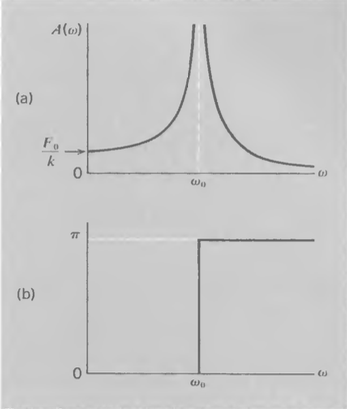
\includegraphics[scale=0.7]{phys232/Ch4-forced-no-damping-A.png} \caption{(a) Absolute amplitude of forced oscillations (no damping) as a function of $\omega$; (b) phase lag of $x$ with respect to the driving force, as a function of $\omega$.}	\label{ch4:no-damping-A}
\end{figure}
\end{proof}

\subsection{Resonant response, using complex exponentials}
Recall \eqref{ch4:eq-no-b}:
\[ m\ddot{x} + kx = F_0 \cos(\omega t) \]

Visualize the driving force $F_0 \cos(\omega t)$ as the real component of $F_0 e^{j\omega t}$.

Assume $x$ is the real part of a rotating vector $z$, such that:
\[ m\ddot{z} + kz = F_0 e^{j\omega t}\]

Assume the following solution:
\[z = Ae^{j(\omega t+\alpha)} \]

Substitute in \eqref{ch4:eq-acc-forced-no-b}:
\begin{align*}
	(-m\omega^2 A + kA)e^{j(\cancel{\omega t} + \alpha)} &= F_0 \, \cancel{e^{j\omega t}} \\
	A(-\omega^2 + \omega_0^2)e^{j\alpha} &= \frac{F_0}{m} \\
	A(\omega_0^2 - \omega^2 ) &= \frac{F_0}{m} e^{-j\alpha} \\
	\Longrightarrow
	\underbrace{A(\omega_0^2 - \omega^2 )}_\text{real} &= \underbrace{\frac{F_0}{m} \cos\alpha}_\text{real} - \underbrace{j\frac{F_0}{m} \sin\alpha}_\text{imaginary}
\end{align*}

Comparing the real and imaginary components on each side:
\begin{align*}
	\text{Real part: } & A(\omega_0^2 - \omega^2 ) = \frac{F_0}{m} \cos\alpha \\
	\text{Imaginary part: } & \frac{F_0}{m} \sin\alpha = 0 
\end{align*}

From the imaginary part, $\alpha = n\pi, n\in\mathbb{Z}$. From the real part, we obtain:
\begin{align*}
	A(\omega_0^2 - \omega^2 ) &= \frac{F_0}{m} \\
	\therefore
	A &= \frac{F_0/m}{\omega_0^2 - \omega^2 }
\end{align*}
which is the same result obtained in \eqref{ch4:soln-no-b}.

\section{Forced Oscillations with Damping: Steady State}

Let us continue to examine only the \emph{steady state}.

Equation of motion:
\[ \ddot{x} + \gamma\dot{x} + \omega_0^2 = F_0 \cos(\omega t) \]

Results: 
\[ x = A \cos (\omega t - \delta) \]
\[ A(\omega) = \frac{F_0/m}{[(\omega_0^2 - \omega^2)^2 + (\gamma\omega)^2]^{1/2}} \]
\[ \tan \delta (\omega) = \frac{\gamma\omega}{\omega_0^2 - \omega^2}\]

Independent of adjustable initial starting conditions!

\subsubsection{Transient Effects}
For $t<0$, let the object be at rest (i.e. it only starts moving at $t=0$).
\begin{align*}
x &= steady + transient \\
x &= A \cos (\omega t - \delta) + B e^{-\gamma t/2} \cos(\omega' + \beta)
\end{align*}

The transient part (system's ''natural" motion) dies out over time due to damping; after then, the steady state takes over. 

Transient part of the equation accounts for adjustable initial conditions!

A \emph{beat pattern} may be produced during this stage if $\omega'$ (system's freq w/ damping) and $\omega$ are similar.

\section{Power}
Power required to keep a driven oscillator going at the same amplitude:
\[ P = \frac{dW}{dt} = F\frac{dx}{dt} = Fv \]
\chapter{Coupled Oscillators \& Normal Modes}



\end{document}